\documentclass[a4paper]{article}
\usepackage{amsfonts}
\usepackage{amsmath}
\usepackage{amssymb}
\usepackage{graphicx}     

\begin{document}
  
\noindent \large Auteur: Stan Van Campenhout \\
\noindent \large Studierichting:  Informatica\\
\noindent \large Oefeningenreeks 5G nr. 11\\

\medskip

\normalsize

\begin{figure}[h]
\centering
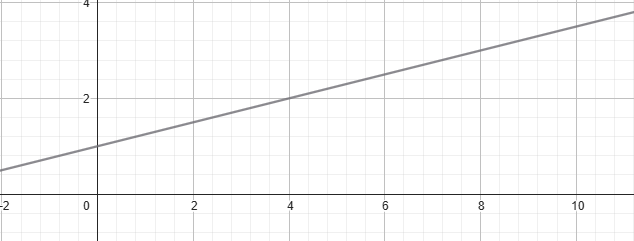
\includegraphics[width=7cm]{5G-11-stan.van.campenhout.INF.png}

\end{figure}

$ y - r = \dfrac{R - r}{h}\left(x-0\right) \Leftrightarrow y = \dfrac{R- r}{h}x + r $\\

$ \Rightarrow \pi\displaystyle\int_0^h\left(\dfrac{R- r}{h}x + r\right)^2dx = \pi\displaystyle\int_0^h\left(\dfrac{R^2-2Rr+r^2}{h^2}x^2 + 2r\dfrac{R-r}{h}x+r^2\right)dx$\\

$ = \pi\dfrac{R^2-2Rr+r^2}{3h^2}\left[x^3\right]_0^h + \pi r\dfrac{R-r}{h}\left[x^2\right]_0^h + \pi r^2\left[x\right]_0^h $\\

$ = \pi h\left(\dfrac{R^2-2Rr+r^2+3Rr-3r^2+3r^2}{3}\right) = \dfrac{1}{3}\pi h\left(R^2+2Rr+r^2\right) $\\

\begin{thebibliography}{999}
%\bibitem{a} Referentie
\end{thebibliography}
\end{document} 
